\documentclass[problems]{esg8022pset} 
\usepackage{amsmath}
\usepackage{amssymb}
\usepackage{enumerate}
\usepackage{graphicx}
\usepackage{hyperref}
\usepackage{mathtools}
\usepackage[per-mode=symbol]{siunitx} %If this line is giving you trouble, try replacing per-mode with per
%use inter-unit-separator={}\cdot{} ?
\providecommand{\uvec}[1]{{\hat{\bf{#1}}}}
\usepackage{pgf,tikz}
\usetikzlibrary{arrows}
\usepackage{wasysym}
\usepackage{subfig}
\makeatletter
\newcommand{\interitemtext}[1]{%
  \begin{list}{}
   {\itemindent=0mm\labelsep=0mm
   \labelwidth=0mm\leftmargin=0mm
   \addtolength{\leftmargin}{-\@totalleftmargin}}
    \item #1
  \end{list}
}
\makeatother
\renewcommand{\d}{\,d}
\providecommand{\norm}[1]{\lVert#1\rVert}

\newcommand{\Kgrad}{\left(\hat{x} \frac{\partial}{\partial x} + \hat{y} \frac{\partial}{\partial y} + \hat{z} \frac{\partial}{\partial z}\right)}
\newcommand{\Kdiv}[6]{{#4}\left(\frac{\partial {#1}}{\partial x} {#5} \frac{\partial {#2}}{\partial y} {#6}\frac{\partial #3}{\partial z} \right)}
\newcommand{\KKdiv}[6]{{#4}\left(\frac{\partial}{\partial x}{#1} {#5} \frac{\partial}{\partial y}{#2} {#6}\frac{\partial}{\partial z}{#3} \right)}
\newcommand{\dx}{\frac{\partial}{\partial x}}
\newcommand{\dy}{\frac{\partial}{\partial y}}
\newcommand{\dz}{\frac{\partial}{\partial z}}
\newcommand{\dtheta}{\frac{\partial}{\partial \theta}}
\newcommand{\dr}{\frac{\partial}{\partial r}}

\AtBeginDocument{%
  % Appologies to any future editor on the inconsistencies in TeX code and the unnecessary braces.  I'm aggregating previously typeset problems, and didn't think it worth my time to improve the quality of TeX code in ways that won't make any difference to the typeset material. -Jason Gross (jgross@mit.edu)
}%
\classname{Physics 8.022} \semester{Spring 2011} 
\problemsetnumber{8}
\date{\today }
\duedate{Tuesday, April 5th at 9 \textsc {pm}}
\readingassignment{}
\problemsettitle{Amp\`{e}re's law, Biot-Savart law}
\begin{document}
\section{Problem \thesection: Long flat conductor}
  A long flat conductor of width $a$ carries a sheet of current $i$ (see
  \autoref{fig:flat}). You are asked to find the magnetic field (direction and
  magnitude) near the center of its flat side and and very close to the
  surface, such that the distance $R$ from the sheet is $R \ll a$.

  \begin{figure}[H]
    \centering
    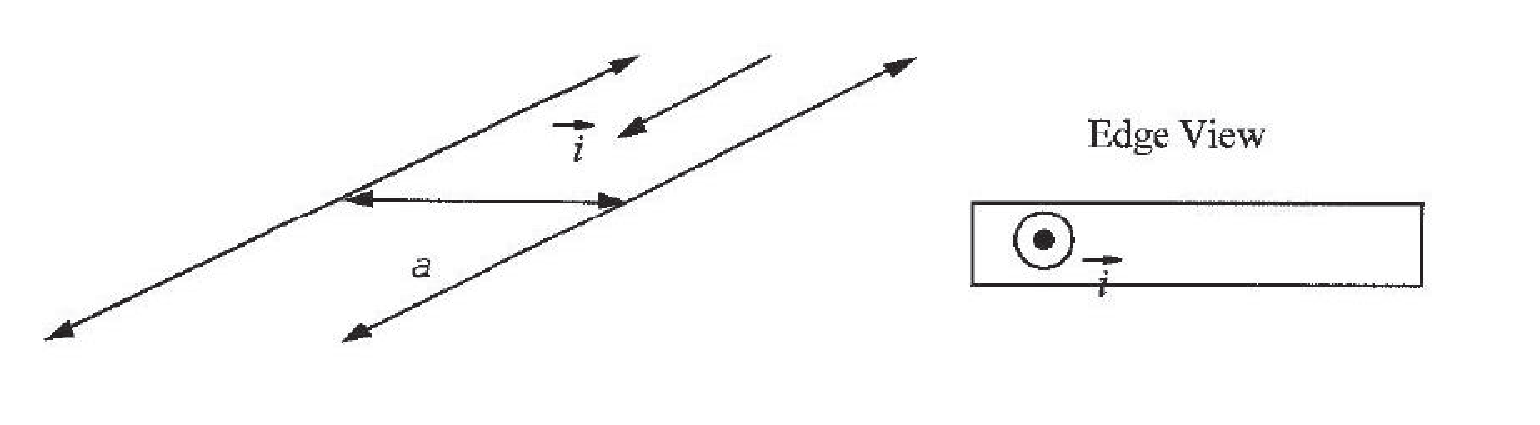
\includegraphics[width = 10cm]{flat_conductor}
    \caption{Flat conductor}
    \label{fig:flat}
  \end{figure}
\section{Problem \thesection: Magnetic field of three wires --- Purcell 6.5}
  Three long straight parallel wires are located as shown in the diagram. One
  wire (B) carries current $2 I$ into the paper; each of the others (A and C)
  carries current $I$ in the opposite direction. What is the strength if the
  magnetic field at $P_1$ and $P_{2}$?
  \begin{figure}[H]
    \centering
    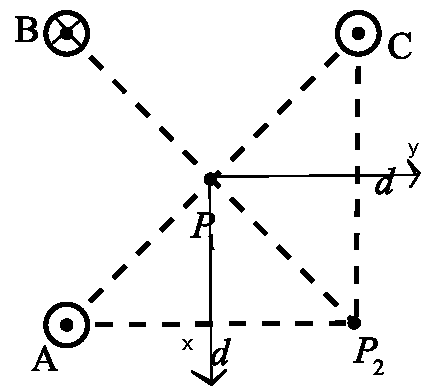
\includegraphics[width = 5cm]{Threewires}
%    \label{fig:threewire} % \label doesn't work without \caption
  \end{figure}
\section{Problem \thesection: Bent wire revisited}
  In class we found the magnetic field at the center of a wire bent through
  $180^\circ$.  Solve it instead for the wire bent through some arbitrary
  angle.
\section{Problem \thesection: Magnetic field due to a spinning disk}
  A flat circular disk with radius $R$ carries a uniform surface charge density
  $\sigma$. It rotates with an angular velocity $\omega$ about the $z$-axis.
  Find the magnetic field $\vec{B}(z)$ at any point $z$ along the rotation
  axis.
  \begin{figure}[H]
    \centering
    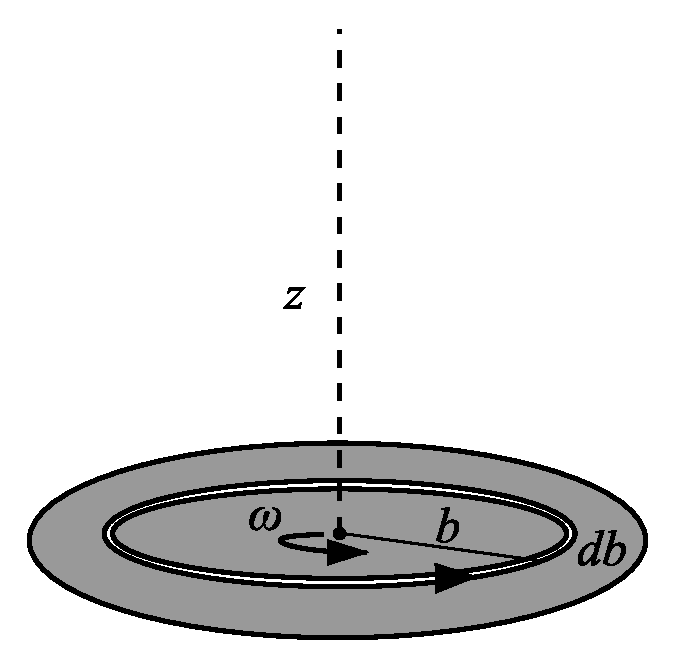
\includegraphics[width = 5cm]{Spinningdisk}
%    \label{fig:spinningdisk} % \label doesn't work without \caption
  \end{figure}
\section{Problem \thesection: Coaxial cable}
  A long coaxial cable consists of two concentric conductors, as shown in
  \autoref{fig:coax} below.  The inner conductor is a cylinder with radius $a$,
  and it carries a current $I$ uniformly distributed over its cross section.
  The outer conductor is a cylindrical shell with inner radius $b$ and outer
  radius $c$. It carries a current $I$ that is also uniformly distributed over
  its cross section, and that is opposite in direction to the current of the
  inner conductor.  Calculate the magnetic field $\vec{B}$  and plot the field
  strength as a function of the distance from the axis.
  \begin{figure}[H]
    \centering
    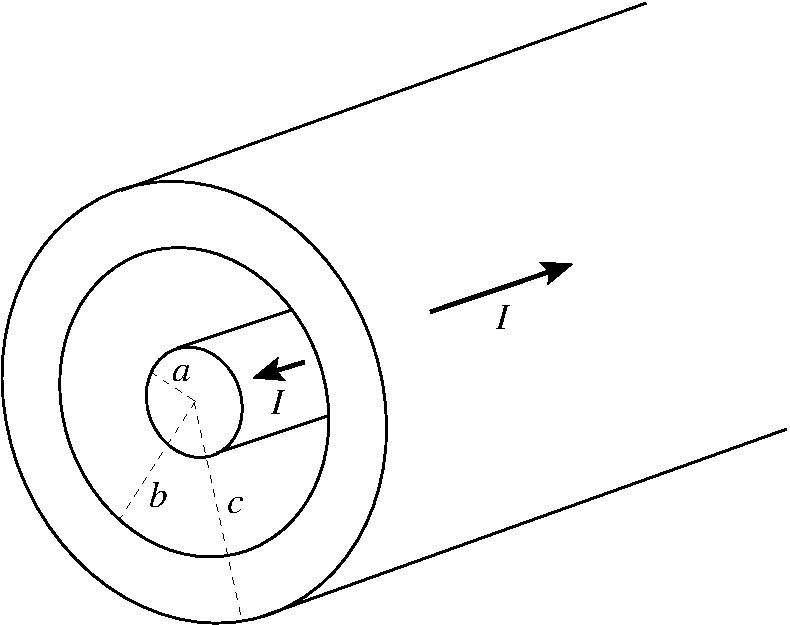
\includegraphics[width = 5cm]{coax}
    \caption{Cross-section of a long coaxial cable.}
    \label{fig:coax}
  \end{figure}
\section{Problem \thesection: Rectangular Toroidal Solenoid --- Purcell 6.14}
  What is the magnetic field inside and outside of the solenoid in \autoref{fig:toroid}?
  \begin{figure}[H]
    \centering
    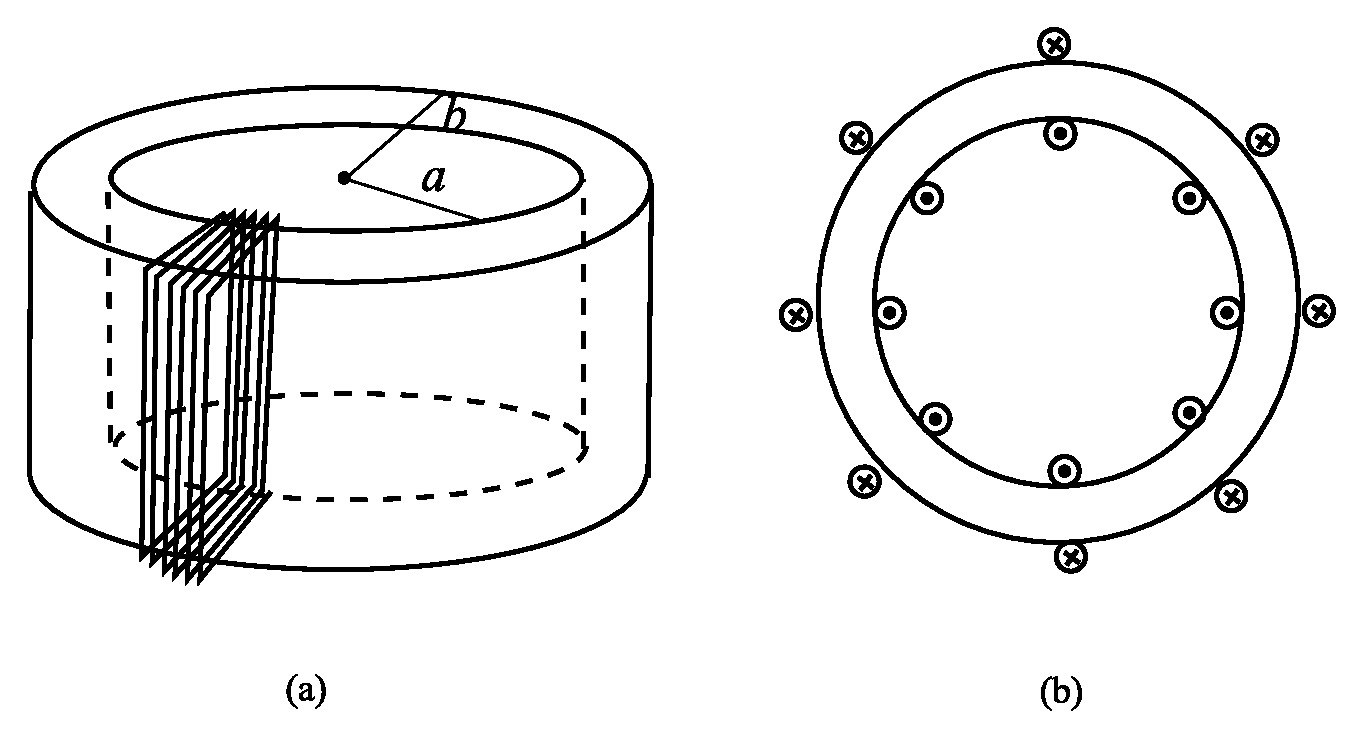
\includegraphics[width = 5cm]{Toroid}
    \caption{A Toroidal Solenoid}
    \label{fig:toroid}
  \end{figure}
\section{Problem \thesection: Vector potential of a solenoid}
  Find the vector potential $\vec A$ inside and outside of an infinite solenoid
  of radius $R$ with $n$ turns per centimeter, each carrying current $I$.  Find
  the solution for $\vec A$ which is symmetric about the axis of the solenoid.

  \noindent \textsc{Hint}: You can come up with a \emph{very} simple way to
  compute $\vec A$ by putting together
  \begin{itemize}
    \item The magnetic flux, $\Phi_B = \int \vec B\cdot d\vec a$
    \item The definition $\vec B = \vec\nabla\times\vec A$
    \item Stoke's theorem.
  \end{itemize}
\section{Problem \thesection: The Director's Challenge --- Extra credit!!!}
  Formulate an interesting problem that relates a topic from 8.022 to your
  intended major or any topic about which you are passionate.  Give references
  to help future students to understand the context.  Try to give a solution.
  Any method, theoretical, analytical, numerical, experimental, is acceptable.
  If you can't give a full solution, outline partial solutions. Enjoy!
\end{document}
